\documentclass[12pt]{article}
\usepackage[margin=2cm, bindingoffset=0cm]{geometry}
%\usepackage[german]{babel} 
\usepackage[english]{babel} %sudo apt-get install texlive-lang-german
\usepackage{hyperref} % web links etc.
\usepackage[parfill]{parskip}
\usepackage[utf8]{inputenc}
\usepackage[dvipsnames]{xcolor}
\usepackage{tcolorbox}
\usepackage{helvet} 
\usepackage{framed}
\usepackage{anyfontsize}
\usepackage{csquotes}
\usepackage{mathrsfs}
\usepackage{physics}
\setcounter{MaxMatrixCols}{16}
\usepackage{amssymb}
\usepackage{MnSymbol}
\MakeOuterQuote{"}
\definecolor{quotecolor}{rgb}{0.8,0.9,1}
\renewcommand{\familydefault}{\sfdefault} 
\setlength\parindent{0pt}
\tcbset{boxrule=0pt,colback=quotecolor,arc=5pt,auto outer arc,left=5pt,right=5pt,boxsep=5pt}
%  width=0.9\textwidth,

\setcounter{secnumdepth}{-1}
\begin{document}
\title{\fontsize{25}{25}\selectfont \textbf{About Psychic and Physical Time} \\
\fontsize{12pt}{12pt}\selectfont (translated from German)}
\author{Harald Rieder}
\date{\today}
\maketitle

%\begin{abstract}

%\end{abstract}

\tableofcontents

\section{Motivation}

With what one has to imagine behind the term \emph{time} actually, mankind has a huge problem in the year 2021. Those who think that things are clear have no problem, but also still nothing understood. Those, who have thought more deeply, disagree, to be read for example in Quanta Magazine in \emph{\href{https://www.quantamagazine.org/a-debate-over-the-physics-of-time-20160719/}{A Debate Over the Physics of Time}}. A short historical outline is given in the article \emph{\href{http://cogsci.uci.edu/~ddhoff/HoffmanTime.pdf}{The Origin Of Time in Conscious Agents}} by Donald D. Hoffman. And he thinks that time must have something to do with mind. That time might have something to do with quantum entanglement in terms of physics is at least guessed at, for example in the article \emph{\href{https://arxiv.org/abs/1310.4691}{Time from Quantum Entanglement}}. But just contemporary physics confronts us with the so-called \emph{\href{https://en.wikipedia.org/wiki/Problem_of_time}{Problem of Time}}. 

This article takes the standpoint that time cannot be understood by ignoring the mind. Starting from known physical terrain, it feels its way out into the unknown with the help of a postulated quantum dynamics, which is supposed to contain the interface to the mind. This dynamics is just a quantum dynamics without Schrödinger dynamics, a pure "collapse" dynamics, and thus in a way the opposite of the \href{https://en.wikipedia.org/wiki/Many-worlds_interpretation}{many-worlds interpretation}.

The success of relativistic physics teaches us that time somehow has to be of equal rank with space. If an observer changes his perspective in a certain way, coordinates which before looked like pure space coordinates suddenly look a little bit like time coordinates, and vice versa. Such a change of perspective is called \emph{Lorentz transformation} in special relativity\footnote{An example from general relativity: When passing the event horizon of the Schwarzschild metric, radial term and time term exchange their signs.}. 

Everyday life shapes in us the idea that time passes continuously and in a certain direction. For everyday events usually do not seem to be reversible. A shattered cup does not reassemble itself into a healthy cup over time and return to the table while cooling down. Such everyday events are modeled by the 2nd law of thermodynamics.

The success of physics as a whole teaches us that position space has no built-in direction. There is no theorem that claims that if you go in a certain direction, the cups must become more and more broken.

Thus we have 3 successfully applicable concepts that seem to be in contradiction. Space and time are like brother and sister. Time has a built-in direction and passes by itself, but space does not. So what?

Therefore we look at what a few unconventional assumptions can lead us to:

\begin{itemize}
\item In physics time does not pass. The nature of physical time is like the nature of physical position space\footnote{Actually, this article considers spacetime as an emergent phenomenon. Like any meaning, the meaning "spacetime" emerges only in a recipient of information. The latter, however, is regarded as physical.}.
\item Time passes in the mind. It is an integral part of conscious becoming. 
\item There must be a mechanism that couples psychic time with a component of the physical world in such a way that, at least for the human mind, it appears that physical time is objectively passing.
\end{itemize}

\section{Idea for a Quantum Clock}

In quantum mechanics events take place in a many-dimensional configuration space, the Hilbert space\footnote{Subtleties like Rigged Hilbert Space or Fock space are not yet of interest in this context.}. A position does not exist in this space at first. Only by fixing on a basis complex-valued functions can be created. These functions stand for infinitely many amplitudes, which are numbered by a continuous real-valued index $x$.

By observation as well as by symmetries which we attribute from experience to a three-dimensional position space, we succeed in the connection. An infinite number of bases can be chosen, but only certain choices lead to an indexing where we can interpret the index as a space coordinate. The scalar product with the abstract vector of a "position base" gives us the amplitude of an abstract state vector $\ket{\psi}$ at a given position
\begin{equation} 
\psi(x) \equiv \bra{x}\ket{\psi} 
\end{equation}
If we want to treat physical time similarly to space, then the time coordinate $t$ must also be a real-valued continuous index. That is
\begin{equation} 
\label{eq:psi_xt}
\psi(t,x) \equiv \bra{t,x}\ket{\psi} 
\end{equation}
The indices $x$ and $t$ now number together a product basis of space and time eigenvectors. We could, due to the equal cardinality\footnote{This is the cardinality of the continuum.} of $\mathbb{R}$ with $\mathbb{R}^2$, replace this index with a common real-valued index $s = s(x,t)$ and again arrive at the form
\begin{equation}
\label{eq:psi_s}
\psi(s) \equiv \bra{s}\ket{\psi} 
\end{equation}
where $\ket{\psi}$ as in (\ref{eq:psi_xt}) would be the abstract state vector in the product space.

We assume that the observer from his Hilbert space $\mathscr{H}_X$ is not able to experience physical time "directly". This assumption is expressed in quantum mechanics in such a way that time does not appear in matrix elements $H(X,x)$ of interaction Hamiltonians. An observer must read a pointer position, a location in space, to infer time in the clock state from there. 

\begin{figure}[!h]\begin{center}
  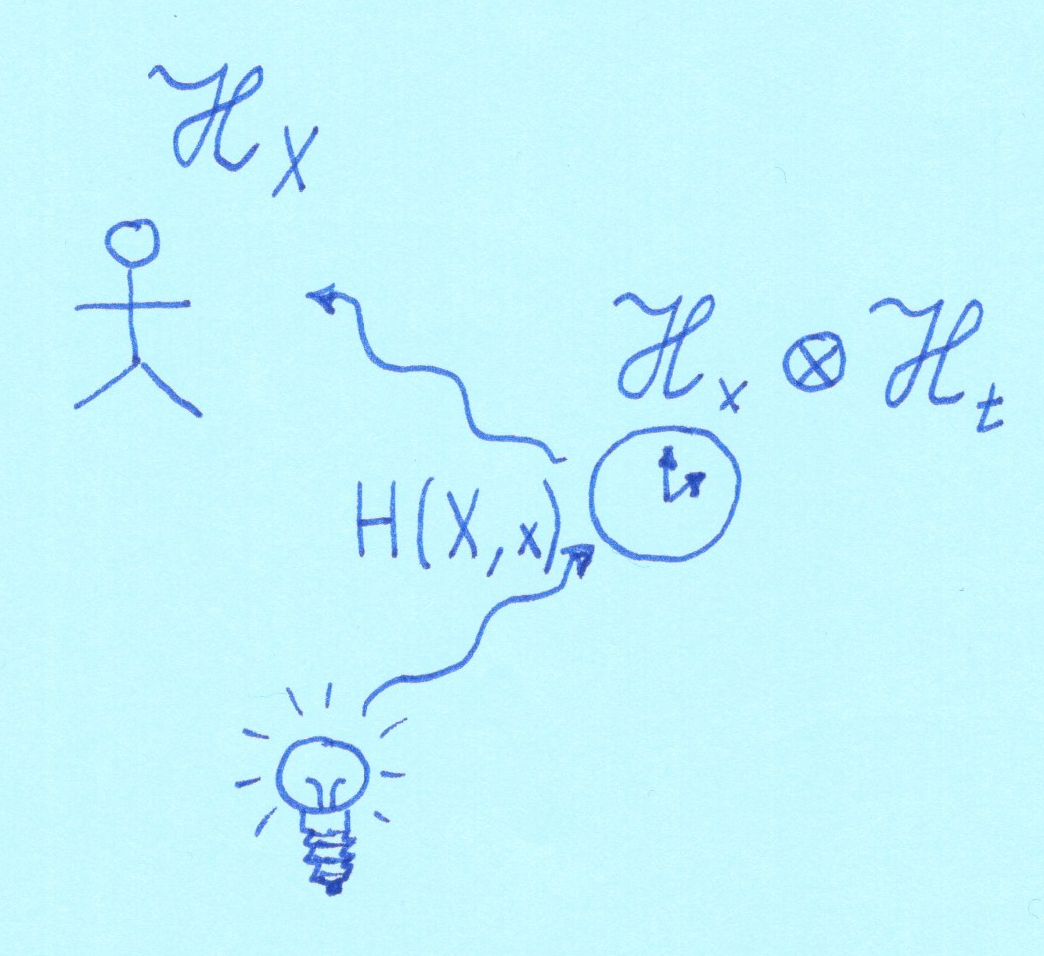
\includegraphics[width=6cm]{Quantenuhr.png}
  \caption{indirect reading of the time}
  \label{fig:clock}
\end{center}\end{figure}

Thus, a good clock state can be a state vector in the product space $\mathscr{H}_x \otimes \mathscr{H}_t$ that maximally entangles space and time subspaces. If $\delta(x-\xi)$ are the amplitudes of position eigenvectors of the position subspace in the position representation, and $\delta(t-\tau)$ are the amplitudes of time eigenvectors of the time subspace in the time representation, then$\footnote{From now on we omit the integral limits if they are at infinity.}$
\begin{equation} 
\label{eq:psi_clock}
\psi(t,x) \sim \int_{-\infty}^{\infty} \mathrm d\chi \, \delta(t-\chi) \delta(x-\chi) = \delta(t-x)
\end{equation}
are the amplitudes of a maximally entangled state that lets us safely infer from the observation of position $\xi$ to time $\tau$. By the observation (or measurement) the superposition "collapses"
\begin{equation} 
\label{eq:collapse}
\int \mathrm d\chi \, \delta(t-\chi) \delta(x-\chi) \quad \rightarrow \quad \delta(t-\chi)\delta(x-\chi)
\end{equation}
This breaks the clock. Because by compatible measurements, i.e. repeated local measurements, we will always encounter only this state and thus the time $\chi$. So there is missing a mechanism which arms the clock again, brings it back into its entangled state.

In the article \emph{\href{https://docs.google.com/document/d/1OrmVETmnBSe5c0CpTbKH8Vq5pWFuB8QUez-KqHTaarQ/edit?usp=sharing}{Ideas about a Quantum Theory without Process Type 2}} such a mechanism is presented. There it is postulated that every conscious observer on the one hand defines a split of the Hilbert space, on the other hand consciously experiences the change of entanglement, as it arises by the split\footnote{technically: Schmidt decomposition} of the current state vector. Possibly the observer can make choices willingly, whereby then \emph{from the point of view of the observer} the quantum mechanical superposition collapses and at the end a pure product state is present. At least 2 such observers (\emph{conscious splits}) connected to the physical channel are necessary to keep events going. This way our clock shall be read "from time to time" by an external observer as shown. So we need another "internal" observer who must split the x,t product space in a different way than the external observer. To do this, the internal observer splits the product space not into x- and t-bases, but into a base of x,t-entangled states and a base containing all the rest.

To see how it works, let's look at a simple example....

\section{A Quantum Clock made of 2 Qutrits}

Our simple quantum clock is supposed to have only 3 discrete pointer positions: $\ket{x=0}, \ket{x=1}, \ket{x=2}$. It shall also be able to measure only 3 time values: $\ket{t=0}, \ket{t=1}, \ket{t=2}$. We will omit x and t later for clarity, x should be on the left, t on the right. That is, for example, $\ket{00}$ should stand for $\ket{x=0}\ket{t=0}$. 

We are dealing with a product space of 2 qutrits, 1 space and 1 time qutrit. Thus, 9 basis vectors are necessary for an orthogonal basis. We build these from the products of the 3 space and 3 time eigenvectors.


For example, we can form an x,t-entangled state like this
\begin{equation*}
\frac{1}{\sqrt{2}} \left(\, \ket{x=0}\otimes\ket{t=0} + \ket{x=1}\otimes\ket{t=1} \,\right) \equiv 
\frac{1}{\sqrt{2}} \left(\, \ket{00} + \ket{11} \,\right)
\quad\quad\hat{=}\quad\quad
\frac{1}{\sqrt{2}}
\begin{pmatrix}
1 \\ 0 \\ 0 \\ 0 \\ 1 \\ 0 \\ 0 \\ 0 \\ 0 
\end{pmatrix}
\quad
\begin{matrix}
00 \\ 01 \\ 02 \\ 10 \\ 11 \\ 12 \\ 20 \\ 21 \\ 22 
\end{matrix}
\end{equation*}
and an unentangled state like this
\begin{equation*}
\frac{1}{\sqrt{2}}\, \ket{x=1}\otimes \left(\,\ket{t=0} + \ket{t=2} \,\right) \equiv 
\frac{1}{\sqrt{2}} \left(\, \ket{10} + \ket{12} \,\right)
\quad\quad\hat{=}\quad\quad
\frac{1}{\sqrt{2}}
\begin{pmatrix}
0 \\ 0 \\ 0 \\ 1 \\ 0 \\ 1 \\ 0 \\ 0 \\ 0 
\end{pmatrix}
\quad
\begin{matrix}
00 \\ 01 \\ 02 \\ 10 \\ 11 \\ 12 \\ 20 \\ 21 \\ 22 
\end{matrix}
\end{equation*}
This is the perspective of the external observer. The clock is supposed to offer him entangled states composed of linear combinations of $\ket{\chi\chi}$ vectors. He then chooses one of the vectors with a probability according to Born's rule. 

Thereupon the clock has to be armed again, for which we need the internal observer. For the internal observer, all $\ket{\chi}_{ext}$ states must look entangled for him to act. To switch to his perspective, we need a unitary matrix $U$ in the product space, for example\footnote{We now omit elements with value 0 more often for clarity.}.
\begin{equation}
U\ =\ 
\begin{pmatrix}
\label{eq:U}
\pmb{a_0} &&&&& \pmb{a_2} &&&&& \pmb{a_1} \\
  & 1 &   &   &   &   &   &   &   &   &   \\
  &   & 1 &   &   &   &   &   &   &   &   \\
  &   &   & 1 &   &   &   &   &   &   &   \\
\pmb{a_1} &&&&& \pmb{a_0} &&&&& \pmb{a_2} \\
  &   &   &   &   &   & 1 &   &   &   &   \\
  &   &   &   &   &   &   & 1 &   &   &   \\
  &   &   &   &   &   &   &   & 1 &   &   \\
\pmb{a_2} &&&&& \pmb{a_1} &&&&& \pmb{a_0} \\
\end{pmatrix}
\quad
\begin{matrix}
00 \\ 01 \\ 02 \\ 10 \\ 11 \\ 12 \\ 20 \\ 21 \\ 22 
\end{matrix}
\end{equation}
The complex values $a_0$, $a_1$, $a_2$ at the places representing x,t-entanglement rotate their places in the 3 affected column vectors and also in the affected row vectors. The values are to be chosen appropriately, which we will come to.

For example, if the external observer has measured time t=0, then the clock is in state $\ket{00}_{ext}$. This state, from the point of view of the internal observer, is an entanglement of $\ket{00}_{int}$, $\ket{11}_{int}$, and $\ket{22}_{int}$.\footnote{We do not know what meaning the pairs of digits have for him.}. With Born's probabilities, the superposition collapses from his point of view:
\begin{equation*}
\begin{matrix}
\ket{00}_{ext} \ \xrightarrow{U} \ a_0\ket{00}_{int} + a_1\ket{11}_{int} + a_2\ket{22}_{int} 
& \xrightarrow{p = |a_0|^2} & \ket{00}_{int} \\ \\
& \xrightarrow{p = |a_1|^2} & \ket{11}_{int} \\ \\
& \xrightarrow{p = |a_2|^2} & \ket{22}_{int}
\end{matrix}
\end{equation*}
In order for the process to continue, we need the external observer again. The inverse of $U$ transforms back to his view and makes unentangled internal states $\ket{\chi\chi}_{int}$ appear entangled.
\begin{equation}
U^{-1}\ =\ 
\begin{pmatrix}
\label{eq:not_U}
\pmb{a_0} &&&&& \pmb{a_1} &&&&& \pmb{a_2} \\
  & 1 &   &   &   &   &   &   &   &   &   \\
  &   & 1 &   &   &   &   &   &   &   &   \\
  &   &   & 1 &   &   &   &   &   &   &   \\
\pmb{a_2} &&&&& \pmb{a_0} &&&&& \pmb{a_1} \\
  &   &   &   &   &   & 1 &   &   &   &   \\
  &   &   &   &   &   &   & 1 &   &   &   \\
  &   &   &   &   &   &   &   & 1 &   &   \\
\pmb{a_1} &&&&& \pmb{a_2} &&&&& \pmb{a_0} \\
\end{pmatrix}
\quad
\begin{matrix}
00 \\ 01 \\ 02 \\ 10 \\ 11 \\ 12 \\ 20 \\ 21 \\ 22 
\end{matrix}
\end{equation}
Altogether, we now have a stochastic process. The absolute squared elements of $U$ and $U^{-1}$ give us the probabilities for state transitions. Only the bold elements in (\ref{eq:U}) and (\ref{eq:not_U}) contribute to what happens when we start with $\ket{\chi\chi}_{ext}$ states. We can thus omit the other elements and get smaller 3x3 matrices. If we still combine internal and external view in a 6-component vector, we can specify an \emph{unistochastic} matrix $P$ describing the process which is populated by Born probabilities.
\begin{equation}
P\, =\,
\begin{pmatrix}
0 & \{|U_{ji}|^2\} \\
\{|U_{ij}|^2\} & 0
\end{pmatrix}
\end{equation}
In our example, if we abbreviate $|a_i|^2$ by $p_i$, the stochastic matrix is
\begin{equation}
P\, =\,
\begin{pmatrix}
&&& p_0 & p_1 & p_2 \\
&&& p_2 & p_0 & p_1 \\
&&& p_1 & p_2 & p_0 \\
p_0 & p_2 & p_1 &&& \\
p_1 & p_0 & p_2 &&& \\
p_2 & p_1 & p_0 &&& 
\end{pmatrix}
\quad
\begin{matrix}
00_{ext} \\ 11_{ext} \\ 22_{ext} \\ 00_{int} \\ 11_{int} \\ 22_{int}
\end{matrix}
\end{equation}
The square of the matrix $P$, i.e. $Q:=P^2$, means a change to the internal view and back again. It stands for one tick of time and provides the probabilities with which the external observer observes a certain x,t-entangled state after the tick as a function of the state before the tick.

We now choose concrete numerical values for the clock. The appendix shows how to arrive at suitable values.
\begin{equation*}
a_0=N\frac{sin(\alpha_0+\alpha_1)}{sin(\alpha_1-2\alpha_0)}e^{\mathrm{i}\alpha_0} \quad
a_1=N\frac{sin(\alpha_0+\alpha_1)}{sin(\alpha_0-2\alpha_1)}e^{\mathrm{i}\alpha_1} \quad
a_2=N
\end{equation*}
with 
\begin{equation*}
N\, = \, \left( 1 +
\frac{sin^2(\alpha_0+\alpha_1)}{sin^2(\alpha_1-2\alpha_0)} +
\frac{sin^2(\alpha_0+\alpha_1)}{sin^2(\alpha_0-2\alpha_1)} \right)^{-\frac{1}{2}}
\end{equation*}
And we choose the angles as
\begin{equation*}
\alpha_0 = \pi / 6 \quad \alpha_1 = \pi / 5 \\ \\
\end{equation*}
This gives us
\begin{equation*}
P\, \approx\,
\begin{pmatrix}
   &&& 0.63787 &  0.12644 &  0.23569 \\
   &&& 0.23569 &  0.63787 &  0.12644 \\
   &&& 0.12644 &  0.23569 &  0.63787 \\
   0.63787 &  0.12644 &  0.23569 &&& \\
   0.23569 &  0.63787 &  0.12644 &&& \\
   0.12644 &  0.23569 &  0.63787 &&& 
\end{pmatrix}
\quad
\begin{matrix}
00_{ext} \\ 11_{ext} \\ 22_{ext} \\ 00_{int} \\ 11_{int} \\ 22_{int}
\end{matrix}
\end{equation*}
and
\begin{equation*}
Q=P^2\, \approx\,
\begin{pmatrix}
   0.47841 & 0.26079 & 0.26079 &&& \\
   0.26079 & 0.47841 & 0.26079 &&& \\
   0.26079 & 0.26079 & 0.47841 &&& \\
   &&& 0.47841 & 0.26079 & 0.26079 \\
   &&& 0.26079 & 0.47841 & 0.26079 \\
   &&& 0.26079 & 0.26079 & 0.47841
\end{pmatrix}
\quad
\begin{matrix}
00_{ext} \\ 11_{ext} \\ 22_{ext} \\ 00_{int} \\ 11_{int} \\ 22_{int}
\end{matrix}
\end{equation*}
Expectation values for the observed time can be built like this
\begin{equation*}
<t> = t \cdot Q \cdot \psi \quad\quad t = \begin{pmatrix}
0&1&2&0&0&0
\end{pmatrix}
\end{equation*}
In our example, depending on the initial state, the expectation values are as follows
\begin{center}
\begin{tabular}{ |c|c| } 
 \hline
 $\psi$ & $<t>$ \\ 
 \hline
 $\ket{00}_{ext}$ & 0.78 \\ 
 $\ket{11}_{ext}$ & 1.00 \\ 
 $\ket{22}_{ext}$ & 1.22 \\
 \hline
\end{tabular}
\end{center}
A macroscopic clock, averaging over many quantum clocks, would give us these time values. Starting from t=0 the measured time would run already once forward! If we could handle with very large matrices $U$, then we could possibly create large areas in which the time, better said the quantity which the external observer interprets as time, would run with every mental tick in the same direction.

Larger double-stochastic matrices might still be easy to arrange for this purpose. However, the question whether they are also unistochastic is unfortunately hardly answerable from a row number of 5 on and the present state of research. But they must be unistochastic if they are to be compatible with quantum mechanics.

\section{Growing Entropy with Psychic Time}

Double-stochastic transition matrices in Markov processes lead to a uniform distribution of probabilities in the limit. But what does this mean in our context?

%The stationary distribution of an irreducible aperiodic finite Markov chain is uniform if and only if its transition matrix is doubly stochastic.

We assume that an observer A in Hilbert space $\mathscr{H}_Y$ observes the system of figure \ref{fig:clock} from the "very outside". 
\begin{figure}[!h]\begin{center}
  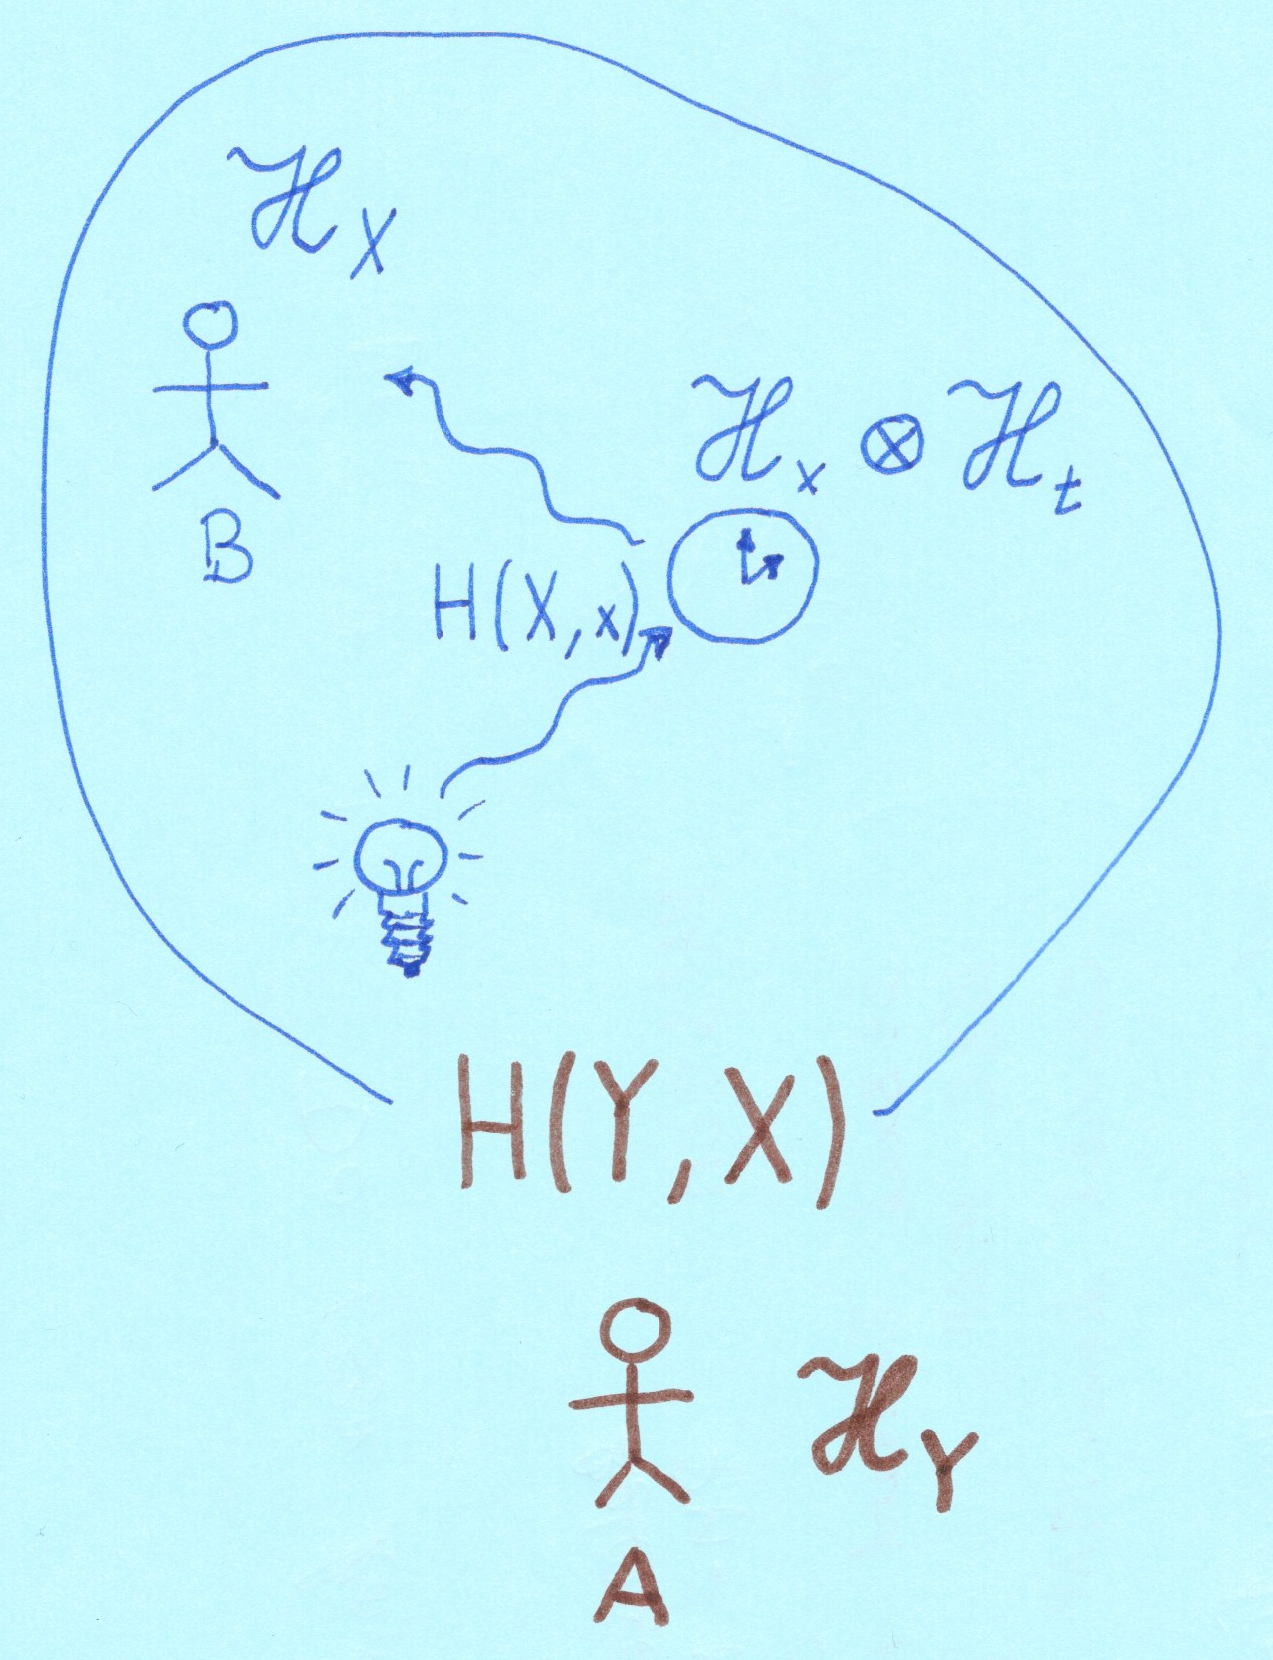
\includegraphics[width=6cm]{Entropie.png}
  \caption{quite external observer}
  \label{fig:entropy}
\end{center}\end{figure}
The observer interacts with her own clocks and thereby experiences a progression of her time. From time to time she couples with an interaction Hamiltonian $H(Y,X)$ to the observer B to ask him about his time. When B replies that he measured $\chi$, she knows that the system is - or just has been - in state\footnote{Here we use $\otimes$ from time to time to denote the dyadic product so that it is clearer what is meant.}
\begin{equation}
\ket{X=\chi}\otimes\ket{\chi\chi}
\end{equation}
The query of the time of B by A is of course also a quantum process. We can think of it as a decoherence process in the limiting case of a quantum measurement. That is, if B has obtained "the knowledge $\chi$", in the ideal case the total state shall be\footnote{For macroscopic observers, we must think of the subspaces of $\mathscr{H}_Y$ and $\mathscr{H}_X$ as strongly degenerate to the measured value $\chi$.}
\begin{equation}
\ket{\Theta}\ \ =\ \ \ket{Y=\chi}\otimes\ket{X=\chi}\otimes\ket{\chi\chi}
\end{equation}
This pure state has entropy 0. Formally, we can form the density operator $\hat{\rho}$ of the system by tracing out the degrees of freedom of Y
\begin{equation}
\hat{\rho}_{\chi,\chi\chi}\ =\ \operatorname{Tr}_Y \ket{\Theta}\bra{\Theta}\ =\ 
\ket{X=\chi}\otimes\ket{\chi\chi}\ \bra{\chi\chi}\otimes\bra{X=\chi} 
\end{equation}
and get for its von-Neumann entropy
\begin{equation}
S\ =\ -\operatorname{Tr} \hat{\rho}_{\chi,\chi\chi} \log_2\ \hat{\rho}_{\chi,\chi\chi}\ = \ 0
\end{equation}
Until the next query $\tau$ ticks shall pass in the system. The matrix $Q$ acts at each tick, so that after $\tau$ ticks, the probabilities for the final states are
\begin{equation}
p_i=\sum_j \{Q^\tau\}_{ij}\, \delta_{j\chi}
\end{equation}
Now we have a mixed state from B's point of view
\begin{equation}
\hat{\rho}_{X,xt}\ = \ \sum_{i=0}^{n-1} p_i \ket{X=i}\otimes\ket{ii}\ \bra{ii}\otimes\bra{X=i} 
\end{equation}
Let $n$ stand for the finite cardinality of the Hilbert space of the system. In the limit $\tau\rightarrow\infty$, the $p_i$ tend to the same value $p_\infty=n^{-1}$, which means the maximization of the von-Neumann entropy of the system. Expressed with the matrix elements of $\hat{\rho}_{X,xt}$.
\begin{equation}
S_\infty\ =\ -\operatorname{Tr} \left(
\begin{pmatrix}
p_\infty&0&\cdots &0\\
0&p_\infty&\cdots &0\\
\vdots &\vdots &\ddots &\vdots \\
0&0&\cdots &p_\infty
\end{pmatrix}
\log_2
\begin{pmatrix}
p_\infty&0&\cdots &0\\
0&p_\infty&\cdots &0\\
\vdots &\vdots &\ddots &\vdots \\
0&0&\cdots &p_\infty
\end{pmatrix} \right)
\ =\ - n \cdot n^{-1} \log_2{n^{-1}} = \log_2{n}
\end{equation}
Now we come back to our simple example and see how the probabilities for the final states evolve after an initial state $\ket{00}$\footnote{Program code can be found in the appendix.}.
\begin{center}
\begin{tabular}{ |c|c|c|c|c|c| } 
 \hline
 $\tau$ & 1 & 2 & 3 & $\cdots$ & $\infty$ \\ 
 $p_0$ & 0.47841 & 0.36491 & 0.34020 & $\cdots$ & 1/3 \\
 $p_1$ & 0.26079 & 0.31755 & 0.32990 & $\cdots$ & 1/3 \\
 $p_2$ & 0.26079 & 0.31755 & 0.32990 & $\cdots$ & 1/3 \\
 \hline
\end{tabular}
\end{center}
By abandoning quantum mechanical processes of type 2, that is, by restricting ourselves to unistochastic processes of type 1, we get increasingly mixed states as time grows. We get a direction in psychic time in which entropy grows without the physical coordinate t having to be given a direction for it. In processes of type 2, Schrödinger dynamics, the entropy depends quasiperiodically on the (physical) time\footnote{See appendix.}.

\section{More Space Dimensions}

The question arises how an x,t-entangled state of the type (\ref{eq:psi_clock}) must be extended to more continuous space dimensions. The answer is found starting from an example in discrete Hilbert space.
\begin{center}
\begin{tabular}{ |c|c|c|c|c| } 
 \hline
 t & x & y & z & s \\ 
 $\ket{t=0}$ & $\ket{x=0}$ & $\ket{y=0}$ & $\ket{z=2}$ & $\ket{s=0}$  \\
 $\ket{t=1}$ & $\ket{x=0}$ & $\ket{y=1}$ & $\ket{z=3}$ & $\ket{s=1}$  \\
 $\ket{t=2}$ & $\ket{x=1}$ & $\ket{y=2}$ & $\ket{z=4}$ & $\ket{s=2}$  \\
 $\vdots$ & $\vdots$ & $\vdots$ & $\vdots$ & $\vdots$ \\
 \hline
\end{tabular}
\end{center}
After a reindexing $u: \mathbb{R}^3 \rightarrow \mathbb{R}, (x,y,z) \mapsto s$, $s$ corresponds to a path parameter. Thus, the generalization of (\ref{eq:psi_clock}) is a state of the type (\ref{eq:psi_s}) $\delta(t-s)$ where $s$ is a path parameter.

Formally, with the choice $t(s) = s$ we can write
\begin{equation} 
\begin{split}
\label{eq:psi_clock_3d_space}
\psi(t,x,y,z) \sim \int \mathrm ds \, \delta(t-s) \, \delta(x-x(s)) \, \delta(y-y(s)) \, \delta(z-z(s)) = 
\\
\delta(x-x(t)) \, \delta(y-y(t)) \, \delta(z-z(t)) \ \hat{=}\ \delta(t-s(x,y,z))
\end{split}
\end{equation}
Any world line that does not intersect itself when projected onto three-dimensional position space is a good clock state. 

\section{A Quantum Clock in Relative Motion}

We now ask how a moving clock is seen, or equivalently, how a clock is seen from a moving observer. 

The operator $\hat{U}$ transforms from the view of the external observer to the view of the internal observer. The operator $\hat{U}^{-1}$ transforms back again.
\begin{figure}[!h]\begin{center}
  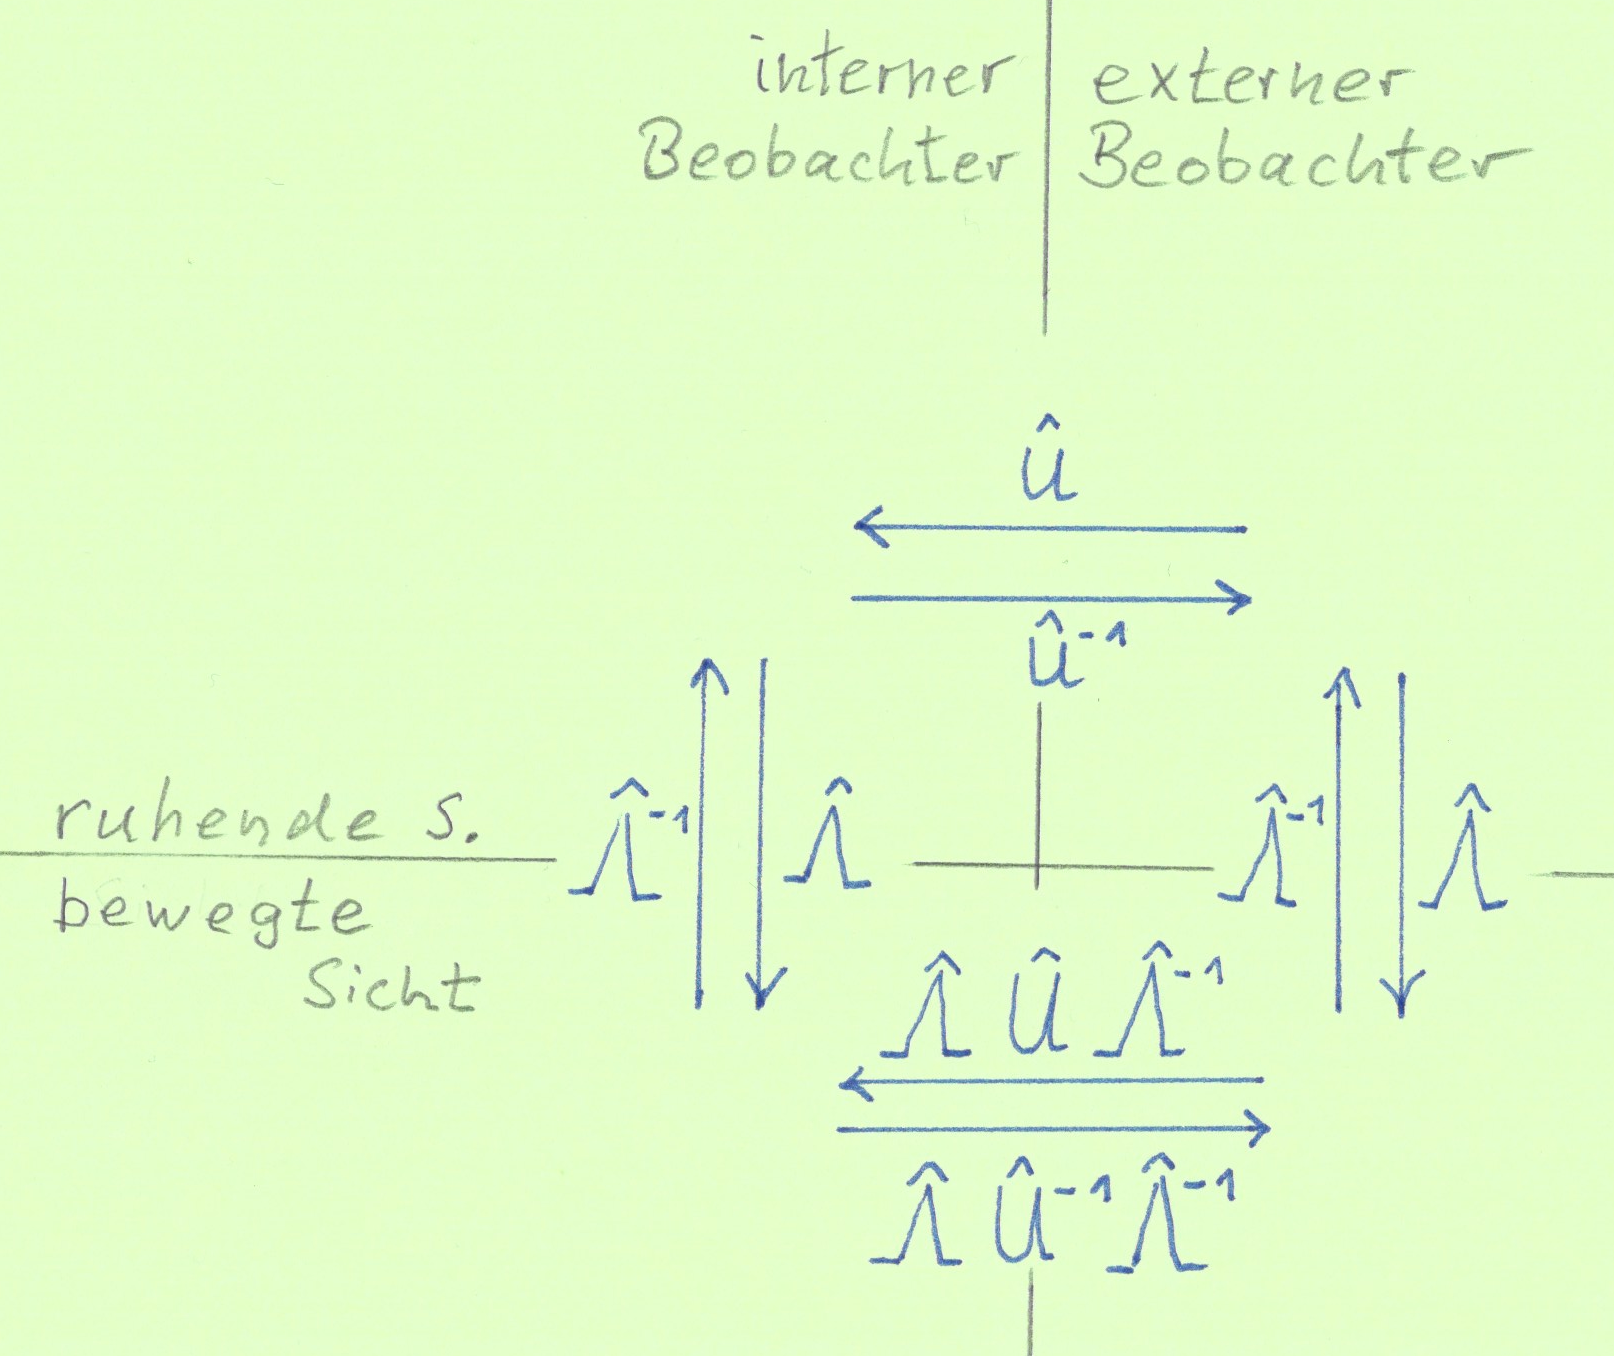
\includegraphics[width=10cm]{Bewegte_Uhr.png}
  \caption{Four different views on a state}
  \label{fig:moved_clock}
\end{center}\end{figure}

A Lorentz boost in x-direction $\hat{\Lambda}_\beta$, parameterized with velocity $\beta=v/c$ transforms states\footnote{We restrict ourselves here to scalar $\psi$.} to the view of a moving observer. The inverse transformation is $\hat{\lambda}_{-\beta} \equiv \hat{\lambda}_{\beta}^{-1}$.

From the figure \ref{fig:moved_clock} we read how the moving observer sees the relation between external and internal observer: it is given by the linear operator $\hat{V} = \hat{\Lambda} \hat{U} \hat{Lambda}^{-1}$. So, in general, the moving observer sees the relation between internal and external observer differently than a stationary observer. Only if $\hat{\Lambda}$ and $\hat{U}$ would commute the relation would appear the same. As we have seen above, this relation determines the progression of physical time with psychic time ticks. So, subjectively, the moving observer generally sees a different progression of physical time with the psychic objective time ticks of the stationary external observer.

A Lorentz boost in x-direction transforms the coordinates according to
\begin{equation*}
\begin{pmatrix} t' \\ x' \end{pmatrix}\ =\ 
\gamma \begin{pmatrix} 1 && -\beta \\ -\beta && 1 \end{pmatrix}
\begin{pmatrix} t \\ x \end{pmatrix}
\end{equation*}
From the condition 
\begin{equation*}
\ket{\psi'}=\hat{\Lambda}\ket{\psi}
\end{equation*}
expressed in components
\begin{equation*}
\psi'(t',x')\ =\ \psi'(\gamma(t-\beta x),\gamma(x-\beta t))\ = \int \mathrm{d}t\,\mathrm{d}x\, \Lambda(t',x',t,x) \psi(t,x)
\end{equation*}
we read off the matrix elements of the Lorentz transformation as
\begin{equation}\label{eq:matrix_elements_Lambda}
\Lambda_\beta(t',x',t,x)\ =\ \delta(t-\gamma(t'+\beta x'))\ \delta(x-\gamma(x'+\beta t'))
\end{equation}
These matrix elements also reflect the concatenation of boosts 
\begin{equation*}
\gamma_3 \begin{pmatrix} 1 && -\beta_3 \\ -\beta_3 && 1 \end{pmatrix} =
\gamma_2 \begin{pmatrix} 1 && -\beta_2 \\ -\beta_2 && 1 \end{pmatrix}
\gamma_1 \begin{pmatrix} 1 && -\beta_1 \\ -\beta_1 && 1 \end{pmatrix}
\end{equation*}
correctly. It is\footnote{See appendix.}
\begin{equation} \label{eq:chained_boosts}
\Lambda_{\beta_3}(t',x',t,x)\ =\ \int \mathrm{d}t''\,\mathrm{d}x''\, \Lambda_{\beta_2}(t',x',t'',x'')\, \Lambda_{\beta_1}(t'',x'',t,x)
\end{equation}
Using (\ref{eq:matrix_elements_Lambda}) we can specify the matrix elements of $\hat{U}$ as seen by the moving observer.
\begin{equation}
\begin{gathered}
V(t_{int}',x_{int}',t_{ext}',x_{ext}')\ =\ \\
\int \mathrm{d}t_{int}''\,\mathrm{d}x_{int}''\, \mathrm{d}t_{ext}''\,\mathrm{d}x_{ext}''\, 
\Lambda_\beta(t_{int}',x_{int}',t_{int}'',x_{int}'') 
U(t_{int}'',x_{int}'',t_{ext}'',x_{ext}'') 
\Lambda_{-\beta}(t_{ext}'',x_{ext}'',t_{ext},x_{ext})
\end{gathered}
\end{equation}
As expected, the following results after insertion of (\ref{eq:matrix_elements_Lambda})
\begin{equation}
V(t_{int}',x_{int}',t_{ext}',x_{ext}')\ =\ 
U(\gamma(t_{int}'-\beta x_{int}'),
\gamma(x_{int}'-\beta t_{int}'),
\gamma(t_{ext}'-\beta x_{ext}'),
\gamma(x_{ext}'-\beta t_{ext}')) 
\end{equation}
The matrix elements of $\hat{U}$ would be invariant under Lorentz boosts if they depended only on the invariant scalars $\sqrt{t_{int}^2-x_{int}^2}$ and $\sqrt{t_{ext}^2-x_{ext}^2}$. The matrices (\ref{eq:U}), which could explain us an increase of entropy with time, do not look like that\footnote{Apart from the fact that they are discrete and not continuous.}. So, at this point one can hope to find Lorentz-\emph{variant} $\hat{U}$ which could explain both an increase of entropy with time and a collapse of the clock process at $\beta=1$.

%\section{Relativistische Ontologie}

%Wenn wir eine verdrehte Sicht einnehmen, erscheint uns die Welt anders, verdreht. Dennoch glauben wir, dass die Welt nach wie vor die gleiche geblieben ist, uns nur anders erscheint. Im mathematischen Modell drückt sich dies so aus, dass bei einer Rotation Koordinaten transformiert werden. Die rotierten Koordinaten (x',y',z') sollen aber dieselben Punkte P im Raum bezeichnen wie die ursprünglichen (x,y,z). Das heißt, wir glauben an eine dauerhafte gleichbleibende Existenz des Raumes und an die dauerhafte gleichbleibende Existenz von Punkten P im Raum. 

%Wenn wir eine gleichförmig relativbewegte Sicht einnehmen, erscheint uns die Welt anders, hyperbolisch verformt. Um konsistent zu bleiben, sollten wir nun auch glauben, dass die Welt die gleiche geblieben ist. Im mathematischen Modell drückt sich dies so aus, dass bei einem Lorentz-Boost Koordinaten transformiert werden. Die transformierten Koordinaten (t',x',y',z') sollen aber dieselben Ereignisse E der Raumzeit bezeichnen wie die ursprünglichen (t,x,y,z). Das heißt, wir müssen dann auch an eine dauerhafte gleichbleibende Existenz der Raumzeit und an die gleichbleibende dauerthafte Existenz aller Ereignisse E glauben. Das hieße also: Ereignisse ereignen sich nicht in der physikalischen Zeit. Ereignisse sind immer schon zu allen erdenklichen Raumzeitpunkten da.

%Die andere Möglichkeit konsistent zu bleiben hieße, den Glauben an die absolute Existenz von Punkten und damit von Raum aufzugeben. Also müssten Punkte im Raum wie Raumzeitpunkte in der Raumzeit erst durch ihr Auftreten in Erscheinung treten. 

%Wird weiter ausgeführt...

%S-Matrix enthält Prozess 1 (außen) und Prozess 2 (mittendrin/Propagator)

\section{Conclusion}

While \emph{\href{https://docs.google.com/document/d/1OrmVETmnBSe5c0CpTbKH8Vq5pWFuB8QUez-KqHTaarQ/edit?usp=sharing}{Ideas about a Quantum Theory without Process Type 2}} has shown the way how a Schrödinger dynamics can approximately emerge from a "collapse" dynamics, this article has shown how, with a different \emph{relative} arrangement of the mental actors, a stochastic dynamics can emerge where time and entropy values grow together. While elsewhere\footnote{See, e.g. \emph{\href{https://arxiv.org/abs/1905.03841}{Classical dynamical coarse-grained entropy and comparison with the quantum version}} from 2020.}  trying to to explain a growth of entropy by means of a subjective coarse-graining, the approach here explains the growth of entropy on an elementary level, so to speak, on the level of a fine-graining, which we presumably have to look for on the Planck scale.

An outlook was given on how one might find a connection between a fine graining and the limiting velocity $\beta$ for information propagation, perhaps without having to resort to general relativity. A challenge will be to connect the mathematical framework of relativity, which is on the stage of a continuum, with a theory of discrete information units.

\newpage
\section{Appendix A: Calculation of the matrix elements of U}

We care here only about the $a_i$ and compress $U$ to a 3x3 matrix. Without restriction on generality, one of the elements can be chosen to be real. We make the approach
\begin{equation*}
U\, =\, N \, 
\begin{pmatrix}
r_0 e^{\mathrm i\alpha_0} & 1 & r_1 e^{\mathrm i\alpha_1} \\
r_1 e^{\mathrm i\alpha_1} & r_0 e^{\mathrm i\alpha_0} & 1 \\
1 & r_1 e^{\mathrm i\alpha_1} & r_0 e^{\mathrm i\alpha_0}
\end{pmatrix}
\quad N, r_i, \alpha_i \in \mathbb{R}
\end{equation*}
$N$ is a normalization constant yet to be determined. For the column vectors to be pairwise orthogonal, the following must apply
\begin{equation*}
r_0 e^{\mathrm  i\alpha_0} + r_0 r_1 e^{\mathrm i(\alpha_1 - \alpha_0)} + r_1 e^{- \mathrm  i\alpha_1} = 0
\end{equation*}
and therefore 
\begin{equation*}
r_0 = - \frac{r_1 e^{-\mathrm i\alpha_1}}{ e^{\mathrm i\alpha_0} + r_1 e^{\mathrm i(\alpha_1 - \alpha_0)} }
\end{equation*}
According to the prerequisite, this quantity must be real. If we expand with the conjugate complex denominator the denominator becomes real and the numerator becomes
\begin{equation*}
-r_1 \left( e^{-\mathrm i(\alpha_0+\alpha_1)} + r_1 e^{\mathrm i(\alpha_0-2\alpha_1)} \right)
\end{equation*}
For this term to be real, it must be
\begin{equation*}
r_1=\frac{sin(\alpha_0+\alpha_1)}{sin(\alpha_0-2\alpha_1)}
\end{equation*}
Accordingly, one comes to 
\begin{equation*}
r_0=\frac{sin(\alpha_0+\alpha_1)}{sin(\alpha_1-2\alpha_0)}
\end{equation*}
and thus for the normalization constant to 
\begin{equation*}
N\, = \, \left( 1 +
\frac{sin^2(\alpha_0+\alpha_1)}{sin^2(\alpha_1-2\alpha_0)} +
\frac{sin^2(\alpha_0+\alpha_1)}{sin^2(\alpha_0-2\alpha_1)} \right)^{-\frac{1}{2}}
\end{equation*}

\section{Appendix B: Schrödinger Dynamics of Entropy}

% https://de.wikipedia.org/wiki/Zeitentwicklungsoperator
Let $\hat{H}$ be the total Hamiltonian operator of the quantum world. Then its \href{https://de.wikipedia.org/wiki/Zeitentwicklungsoperator}{unitary time evolution operator} transporting states from time $t_0$ to time $t$ is
\begin{equation}
\label{eq:propagator}
\hat{T}=e^{-\frac{\mathrm i}{\hbar}(t-t_0)\hat{H}}
\end{equation}
In our quantum universe, there should be no explicit, i.e. classically externally imposed, dependence on time of the Hamilton operator. If one would encounter such a dependence in the universe, one would have to modify the theory to include this dynamics.

A mixed state of the universe should also not exist. An entanglement to the outside cannot exist by definition, because we want to consider the total world. If there would be a mixed state at the beginning, where an emergence by classical "dicing" must be excluded again, then after some complete "measurement" a pure state would exist immediately and would remain pure forever according to Schrödinger dynamics. 

So we consider the time evolution of the \href{https://de.wikipedia.org/wiki/Entropie#Von-Neumann-Entropie}{von-Neumann entropy} of a pure total state $\hat{\rho}=\ket{\psi}\bra{\psi}$. This state can be represented with any orthonormal basis. We take for this purpose the basis $\{\ket{E_i}\}$ of the eigenvectors of $\hat{H}$ to the eigenvalues $E_i$.
\begin{equation}
\label{eq:psi_energy}
\ket{\psi}=\sum_{i}d_{i}\ket{E_i} \quad\quad
\hat{\rho}=\sum_{ij}d_{i}d_{j}^*\, \ket{E_i}\bra{E_j}
\end{equation}
This pure state gets entropy and entanglement by an imaginary split of the total space into the subspaces denoted by X and Y $\mathscr{H} = \mathscr{H}
_X\otimes\mathscr{H}_Y$.

Let $\{\ket{\phi_i}\}$ be a basis in $\mathscr{H}_X$ and $\{\ket{\chi_j}\}$ be a basis in $\mathscr{H}_Y$. The total world state can be built from the product basis $\{\ket{\phi_i}\ket{\chi_j}\}$.
\begin{equation}
\label{eq:psi_product}
\ket{\psi}=\sum_{ij}c_{ij}\, \ket{\phi_i}\ket{\chi_j} \quad\quad
\hat{\rho}=\sum_{ijkl}c_{ij}c_{kl}^*\, \ket{\phi_i}\ket{\chi_j}\bra{\phi_k}\bra{\chi_l}
\end{equation}
Also any energy eigenvector can be build from this (or any other) product basis
\begin{equation}
\label{eq:energy_eigenvector}
\ket{E_i}=\sum_{jk}f_{i\,jk}\, \ket{\phi_j}\ket{\chi_k}
\quad\quad
\bra{E_i}=\sum_{jk}f_{i\,jk}^*\, \bra{\phi_j}\bra{\chi_k}
\end{equation}

The total state (\ref{eq:psi_energy})/(\ref{eq:psi_product}) shall evolve according to Schrödinger dynamics (\ref{eq:propagator})
\begin{equation}
\label{eq:total_dynamic}
\hat{\rho}(\Delta t)=\sum_{ij}d_{i}d_{j}^*\, \hat{T}\, \ket{E_i}\bra{E_j}\, {\hat{T}}^\dagger
= \sum_{ij}d_{i}d_{j}^*\, e^{-\mathrm i \Delta\omega_{ij}\Delta t}\, \ket{E_i}\bra{E_j}
\end{equation}
where we introduced the abbreviations $\Delta t := t-t_0$ and $\Delta \omega_{ij} := \frac{E_i - E_j}{\hbar}$. If we put in the development (\ref{eq:energy_eigenvector}) by the product basis, then (\ref{eq:total_dynamic}) becomes 
\begin{equation*}
\hat{\rho}(\Delta t) = \sum_{ijklmn}d_{i}d_{j}^*\, e^{-\mathrm i \Delta\omega_{ij}\Delta t}\, 
f_{i\,kl}f_{j\,mn}^*\, \ket{\phi_k}\ket{\chi_l}\bra{\phi_m}\bra{\chi_n}
\end{equation*}
To compute the von-Neumann entropy, we first need the density operator of one part, and then compute the entropy by tracing over the other part\footnote{It does not matter which part we choose first, which can be easily shown.}.

This point is quite important ontologically. The entanglement entropy is a property of the relation between parts and cannot be attributed to any part alone, while the entropy of classical thermodynamics is attributed to a part, a "closed system" and it is considered as \href{https://de.wikipedia.org/wiki/Extensive_Gr%C3%B6%C3%9Fe}{extensive quantity growing with volume}. As of 2021, the entropy of black holes is also seen predominantly as a property of a part, the black hole, and not as a property of the relationship between the black hole and the rest of the world, and this despite the fact that the growth of entropy with area at the event horizon is a clear indication of a relational entropy. In case of unequal division into a small space X and a large space Y and in case of discrete spaces, just the cardinality of the small space determines the maximum amount of information which can be exchanged between X and Y. This maximum is flippantly spoken the "number of qubits of X".

We decide to use part X and form its density operator by tracing out over Y using the $\{\ket{\chi_p}\}$
\begin{equation}
\label{eq:rho_quasiperiodic}
\begin{split}
\hat{\rho}_X(\Delta t)
\ = \sum_{ijklmnp}d_{i}d_{j}^*\, e^{-\mathrm i \Delta\omega_{ij}\Delta t} 
f_{i\,kl}f_{j\,mn}^*\, \ket{\phi_k}\bra{\chi_p}\ket{\chi_l}\bra{\phi_m}\bra{\chi_n}\ket{\chi_p}
\\
= \sum_{ijkmp}d_{i}d_{j}^* f_{i\,kp}f_{j\,mp}^*\, e^{-\mathrm i \Delta\omega_{ij}\Delta t} 
\, \ket{\phi_k}\bra{\phi_m} 
\end{split}
\end{equation}
%\ := \sum_{rkm}g_{rkm} e^{-\mathrm i \omega_{r}\Delta t} \hat{P}_{km}
i.e. with the matrix elements
\begin{equation}
\label{eq:rho_matrix_quasiperiodic}
\rho_{km}\ = \sum_{ijp}d_{i}d_{j}^* f_{i\,kp}f_{j\,mp}^*\, e^{-\mathrm i \Delta\omega_{ij}\Delta t} 
\end{equation}
This density operator is quasiperiodic with the frequencies $\Delta \omega_{ij}$. We obtain the entropy by tracing the operator $-\hat{\rho}_X \log_2 \hat{\rho}_X$ with the $\{\ket{\phi_q}\}$
\begin{equation}
\label{eq:S_quasiperiodic}
S = -\sum_q \bra{\phi_q} \hat{\rho}_X(\Delta t) \log_2 \hat{\rho}_X(\Delta t)  \ket{\phi_q}
\end{equation}
or with the matrix elements as
\begin{equation}
\label{eq:S_matrix_quasiperiodic}
S = -\sum_{km}\left(\sum_{ijp}d_{i}d_{j}^* f_{i\,kp}f_{j\,mp}^* e^{-\mathrm i \Delta\omega_{ij}\Delta t}\right)
\log_2 \left(\sum_{i\,jp}d_{i}d_{j}^* f_{i\,mp}f_{j\,kp}^* e^{-\mathrm i \Delta\omega_{ij}\Delta t}\right)
\end{equation}
Now we can see that we could have allowed a mixed world state at the beginning: nothing would have changed in the principal way how the difference frequencies drive the density operator.

In the continuous case analogous happens as with the transition from a Fourier series to the Fourier integral: aperiodic functions can also be represented. 

\section{Appendix C: Example of the Schrödinger dynamics of entropy}
For the simplest possible example, we need a product of 2 qubits.
(\ref{eq:psi_energy}) then becomes
\begin{equation*}
\ket{\psi}\ =\ \begin{pmatrix}
\ket{E_0} & \ket{E_1} & \ket{E_2} & \ket{E_3}
\end{pmatrix}
\cdot
\begin{pmatrix}
d_0 \\ d_1 \\ d_2 \\ d_3 
\end{pmatrix}
\end{equation*}
We now want to split this vector into 2 qubit states according to (\ref{eq:psi_product}).
\begin{equation*}
\ket{\psi}\ =\ \begin{pmatrix}
\ket{\phi_0}\ket{\chi_0} & \ket{\phi_0}\ket{\chi_1} & \ket{\phi_1}\ket{\chi_0} & \ket{\phi_1}\ket{\chi_1}
\end{pmatrix}
\cdot
\begin{pmatrix}
c_{00} \\ c_{01} \\ c_{10} \\ c_{11}
\end{pmatrix}
\end{equation*}
By inserting a unit matrix $ f^\dagger f$ we obtain
\begin{equation*}
\ket{\psi}\ =\ \sum_{i=0}^{3} d_i \ket{E_i} = \sum_{\substack{i=0\\jk=00}}^{\substack{3\\11}} d_i f_{jk\,i}^* f_{i\,jk} \ket{\phi_j}\ket{\chi_k}
\end{equation*}
For the example we take this unitary 4x(2x2) matrix
\begin{equation*}
\begin{matrix}
 & jk & 00\quad \ 01\quad \ 10\quad \ 11 & i \\
f & = & \frac{1}{2}
\begin{pmatrix}
\label{eq:f}
1 & 0 & 1 & \sqrt{2} \\
\sqrt{2} & 1 & 0 & -1 \\
-1 & \sqrt{2} & 1 & 0 \\
0 & -1 & \sqrt{2} & -1
\end{pmatrix} 
& \begin{matrix}0\\1\\2\\3\end{matrix}
\end{matrix}
\end{equation*}
The density matrix (\ref{eq:rho_matrix_quasiperiodic}) is then a 2x2 matrix.

As energy eigenvalues we choose $E_0$ to $E_3$ as 1, 2, 5 and 7 eV to get 6 different difference frequencies. We choose the amplitudes in the same way, so that
\begin{equation*}
\ket{\psi}\ =\ \begin{pmatrix}
\ket{1} & \ket{2} & \ket{5} & \ket{7}
\end{pmatrix}
\cdot \frac{1}{\sqrt{79}}
\begin{pmatrix}
1 \\ 2 \\ 5 \\ 7
\end{pmatrix}
\end{equation*}
\begin{figure}[!h]\begin{center}
  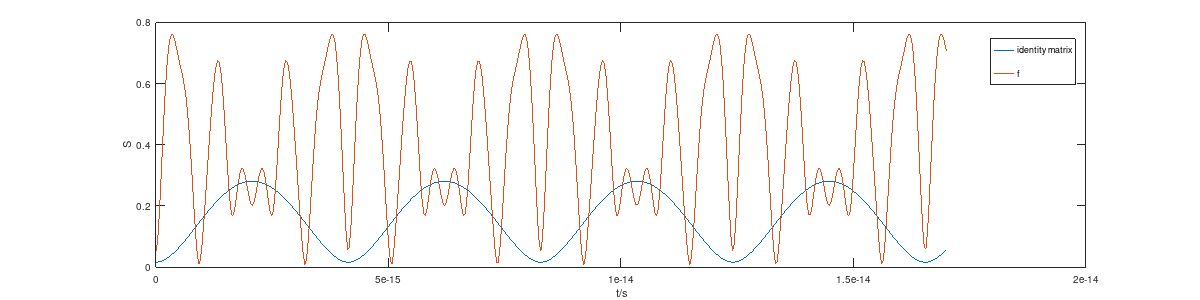
\includegraphics[width=19cm]{periodic_entropy.png}
  \caption{periodic entropy}
  \label{fig:periodic_entropy}
\end{center}\end{figure}

Figure \ref{fig:periodic_entropy} shows the time dependency of entropy with the split $f$. It is strictly periodic since the ratios of the difference frequencies are rational numbers. The periodic duration is about 4.1 femtoseconds.
For reference, the entropy in original view, i.e. with the unit matrix as $f$, was included in the graph (blue).
\begin{figure}[!h]\begin{center}
  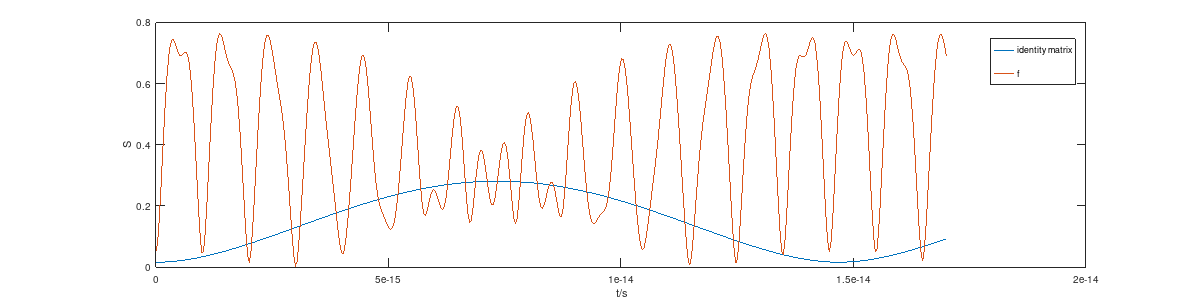
\includegraphics[width=19cm]{quasi_periodic_entropy.png}
  \caption{quasiperiodic entropy}
  \label{fig:quasi_periodic_entropy}
\end{center}\end{figure}

If the ratios of the difference frequencies are no longer all rational numbers, then the time dependency gets quasi-periodic. For figure \ref{fig:quasi_periodic_entropy}, the energy eigenvalue $7$ was replaced by $2.6 \cdot e$. Note that in original view the time dependency is still periodic!

\newpage
\section{Appendix D: Matrix elements of two Lorentz boosts}

Actually it is clear what must come out with the concatenation of the two transformations. Nevertheless, it is written down once explicitly for this example.

(\ref{eq:matrix_elements_Lambda}) inserted into (\ref{eq:chained_boosts}) results in
\begin{equation*}
\begin{gathered}
\Lambda_{\beta_3}(t',x',t,x)\ = 
\\ \\
\int \mathrm{d}t''\,\mathrm{d}x''\,
\delta(t''-\gamma_2(t'+\beta_2 x'))\ \delta(x''-\gamma_2(x'+\beta_2 t'))
\delta(t-\gamma_1(t''+\beta_1 x''))\ \delta(x-\gamma_1(x''+\beta_1 t''))\ =
\\ \\
\int \mathrm{d}x''\,
\delta(x''-\gamma_2(x'+\beta_2 t'))
\delta(t-\gamma_1(\gamma_2(t'+\beta_2 x')+\beta_1 x''))\ \delta(x-\gamma_1(x''+\beta_1 \gamma_2(t'+\beta_2 x')))\ =
\\ \\
\delta(t-\gamma_1(\gamma_2(t'+\beta_2 x')+\beta_1 \gamma_2(x'+\beta_2 t')))\ \delta(x-\gamma_1(\gamma_2(x'+\beta_2 t')+\beta_1 \gamma_2(t'+\beta_2 x')))\ =
\\ \\
\delta(t-\gamma_1\gamma_2((1+\beta_1\beta_2)t'+(\beta_1+\beta_2)x'))\ 
\delta(x-\gamma_1\gamma_2((1+\beta_1\beta_2)x'+(\beta_1+\beta_2)t'))
=
\\ \\
\delta\left(t-\gamma_1\gamma_2(1+\beta_1\beta_2)(t'+\frac{(\beta_1+\beta_2)}{(1+\beta_1\beta_2)}x')\right)\ 
\delta\left(x-\gamma_1\gamma_2(1+\beta_1\beta_2)(x'+\frac{(\beta_1+\beta_2)}{(1+\beta_1\beta_2)}t')\right)
\end{gathered}
\end{equation*}
which is again of the form (\ref{eq:matrix_elements_Lambda}) with the relativistic addition of relative velocities.
\begin{equation*}
\beta_3 = \frac{(\beta_1+\beta_2)}{(1+\beta_1\beta_2)} \quad \quad
\gamma_3 = \gamma_1 \gamma_2(1+\beta_1\beta_2) 
\end{equation*}

\newpage
\section{Appendix E: Gnu Octave Programs}

\subsection{Quantum Clock from 2 Qutrits}
\begin{verbatim}
alpha_0=pi/6;
alpha_1=pi/5;

a_0_abs=sin(alpha_0+alpha_1)/sin(alpha_1-2*alpha_0)
a_1_abs=sin(alpha_0+alpha_1)/sin(alpha_0-2*alpha_1)
a_2_abs=1

a_0=a_0_abs*e^(i*alpha_0);
a_1=a_1_abs*e^(i*alpha_1);
a_2=a_2_abs;

% normalization
N=1/sqrt(a_0_abs^2+a_1_abs^2+a_2_abs^2);

% normalized orthogonal row vectors
u_0=[a_0,a_2,a_1]*N;
u_1=[a_1,a_0,a_2]*N;
u_2=[a_2,a_1,a_0]*N;

% check normalization
u_abs_square=u_0*u_0'

% check orthogonality
u_0_u_1=u_0*u_1'
u_1_u_2=u_1*u_2'
u_2_u_3=u_2*u_0'

% unitary matrix
U=[
u_0;
u_1;
u_2;
]

% null matrix
Null=U-U

% unistochastic matrix
P=[
[Null,U'.*conj(U')];
[U.*conj(U),Null];
]

% one clock tick
P_square=P*P

% external initial states
psi_0=[1,0,0,0,0,0]';
psi_1=[0,1,0,0,0,0]';
psi_2=[0,0,1,0,0,0]';

% time eigenvalues
t=[0,1,2,0,0,0];

% expectation values
exp_t_0 = t*P_square*psi_0
exp_t_1 = t*P_square*psi_1
exp_t_2 = t*P_square*psi_2

% entropy increase with clock ticks
p_1_tick=P_square*psi_0
p_2_ticks=P_square^2*psi_0
p_3_ticks=P_square^3*psi_0
\end{verbatim}

\subsection{Schrödinger Dynamics Entropy}

\begin{verbatim}
# Time evolution of the von Neumann entropy of a 1 qubit density matrix
# according to Schrödinger dynamics.

# example one: energy ratios are rational numbers -> periodic entropy
energies=[1,2,5,7]; # eV

# example two: irrational energy ratios -> quasi periodic entropy
energies2=[1,2,5,2.6*e]; # eV, 1 non-rational number

# example amplitudes of our state vector in energy representation
amplitudes=[1,2,5,7];
# normalize |psi>
amplitudes*=1/sqrt(amplitudes*amplitudes');

# example unitary matrix f, defines the split of the 2 qubit space
f=0.5*[
  1,0,1,sqrt(2);
  sqrt(2),1,0,-1;
  -1,sqrt(2),1,0;
  0,-1,sqrt(2),-1
];
# check unitarity of f
identity=f*f'

# Planck's constant over 2 pi in eV*s units.
function retval = hbar()
  retval = 6.582119569e-16; 
endfunction

# period length of periodic example one
# 1/1, 1/2, 1/3, 1/4, 1/5, 1/6 -> 1/1 common period
printf("period is %10.3e seconds\n",2*pi*hbar); 

# von Neumann entropy of a density matrix with base 2 logarithm
function retval = entropy(matrix)
  retval = -trace(matrix*logm(matrix))*log2(e);
endfunction

#pure_state_density_matrix=amplitudes'*amplitudes
#S=entropy(pure_state_density_matrix)

# Calculates 2x2 density matrix of state |psi> in a 2 qubit space
# depending on the view defined by unitary matrix f and the time.
# f is meant relative to the energy representation.
#
# E_4 vector with 4 energy eigenvalues
# d_4 amplitudes of energy eigenvectors
# (|psi> = sum of d_i * |E_i>)
# f_4_4 4x4 transformation matrix to 2x2 split view
# t time scalar value
function ret = rho_4_4(E_4, d_4, f_4_4, t)
  ret = [0,0;0,0];
  f_adjugate = f_4_4';
  for k_ = 1:2
    for m_ = 1:2
      for i_ = 1:4
        for j_ = 1:4
          omega_ij = (E_4(i_)-E_4(j_))/hbar;
          exp_ij = exp(-i*omega_ij*t);
          for p_ = 1:2
            index_f = (k_-1)*2+(p_-1)+1;
            index_f_adj = (m_-1)*2+(p_-1)+1;
            ret(k_,m_) +=
             d_4(i_)*d_4(j_)'*f_4_4(i_,index_f)*f_adjugate(index_f_adj,j_)*exp_ij;
          endfor
        endfor
      endfor
    endfor
  endfor
endfunction

N_points=500;
t=linspace(0,10.0e-15,N_points); # femto seconds 1e-15
S1=S2=S3=S4=linspace(0,0,N_points);
for t_ = 1:N_points
  rho = rho_4_4(energies, amplitudes, identity, t(t_));
  S = entropy(rho);
  S1(t_) = real(S);
  rho = rho_4_4(energies, amplitudes, f, t(t_));
  #trc=trace(rho) # must be 1
  #trc_square=trace(rho*rho); # must be less or equal 1
  S = entropy(rho);
  S2(t_) = real(S); # suppress imaginary part (numeric errors < 1e-15)
  rho = rho_4_4(energies2, amplitudes, identity, t(t_));
  S = entropy(rho);
  S3(t_) = real(S);
  rho = rho_4_4(energies2, amplitudes, f, t(t_));
  S = entropy(rho);
  S4(t_) = real(S);
endfor
hf=figure(1, 'position', [110 400 1200 400]);
h=plot(t,S1,"-;identity matrix;",t,S2,"-;f;");
xlabel("t/s");
ylabel("S");
print (hf, "periodic_entropy.png", "-dpng","-S1200,400");
hf=figure(2, 'position', [110 40 1200 400]);
h=plot(t,S3,"-;identity matrix;",t,S4,"-;f;");
xlabel("t/s");
ylabel("S");
print (hf, "quasi_periodic_entropy.png", "-dpng","-S1200,400");
\end{verbatim}

\end{document}
